\definecolor{huntergreen}{HTML}{235937}
\definecolor{goldenyellow}{HTML}{FFCC33}
\setbeamercolor{structure}{fg=huntergreen}
\setbeamercolor{palette primary}{fg=huntergreen,bg=goldenyellow}

\logo{\includegraphics[width=0.75in]{img/oswego_logo_horiz_grn}}

\usepackage{amsmath,amssymb,mathtools,physics}


\usepackage{media9}

\newcommand{\playsong}[1]{
\includemedia[
  addresource=#1,
  flashvars={
    source=#1
   &autoPlay=true
  }
]{\fbox{Play}}{APlayer.swf}
}


\usepackage{tikz}
\usetikzlibrary{positioning}
\definecolor{processcolor}{cmyk}{0.96,0,0,0}

\usetikzlibrary{decorations.pathmorphing,shapes}



\newcommand{\markovchain}{
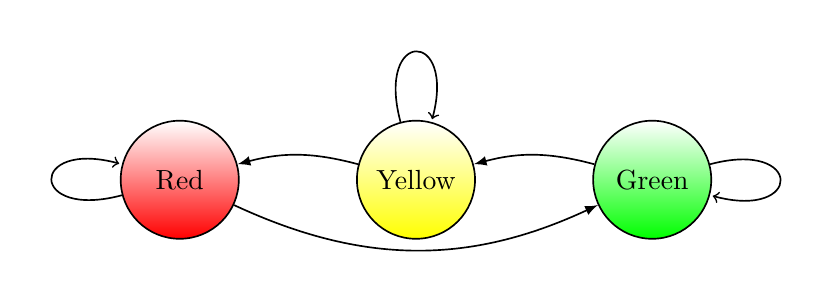
\begin{tikzpicture}[-latex, auto, node distance = 3cm and 3cm, on grid,
                    semithick,
                    state/.style = {circle,
                                    top color = white,
                                    bottom color = black!80,
                                    draw,
                                    black,
                                    text = black,
                                    minimum width = 1.5 cm}]

\node[state] (R) [bottom color = red] {Red};
\node[state] (Y) [bottom color = yellow, right = of R] {Yellow};
\node[state] (G) [bottom color = green, right = of Y] {Green};

\path (G) edge [loop right] (G);
\path (Y) edge [loop above] (Y);
\path (R) edge [loop left]  (R);

\path (G) edge [bend right = 15] (Y);
\path (Y) edge [bend right = 15] (R);
\path (R) edge [bend right = 25] (G);

\end{tikzpicture}
}


\newcommand{\hiddenmarkovmodel}{
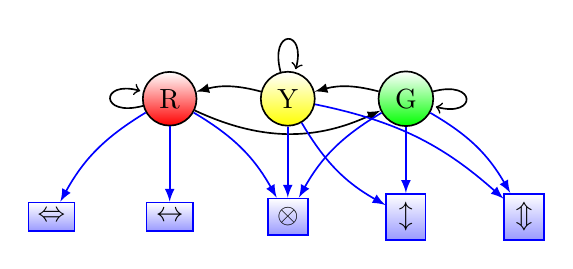
\begin{tikzpicture}[-latex, auto, node distance = 1.5cm and 1.5cm, on grid,
                    semithick,
                    state/.style = {circle,
                                    top color = white,
                                    bottom color = black!80,
                                    draw,
                                    black,
                                    text = black,
                                    minimum width = 0.5 cm},
                    obs/.style   = {rectangle,
                                    top color = white,
                                    bottom color = blue!40,
                                    draw,
                                    blue,
                                    text = black,
                                    minimum width = 0.5 cm}]

\node[state] (R) [bottom color = red] {R};
\node[state] (Y) [bottom color = yellow, right = of R] {Y};
\node[state] (G) [bottom color = green, right = of Y] {G};

\node[obs] (X) [below = of Y] {$\otimes$};
\node[obs] (s) [right = of X] {$\updownarrow$};
\node[obs] (S) [right = of s] {$\Updownarrow$};
\node[obs] (i) [left = of X] {$\leftrightarrow$};
\node[obs] (I) [left = of i] {$\Leftrightarrow$};

\path (G) edge [loop right] (G);
\path (Y) edge [loop above] (Y);
\path (R) edge [loop left]  (R);

\path (G) edge [bend right = 15] (Y);
\path (Y) edge [bend right = 15] (R);
\path (R) edge [bend right = 25] (G);

\path (R) edge [bend right = 15, color = blue] (I);
\path (R) edge [color = blue] (i);
\path (R) edge [bend left = 15, color = blue] (X);

\path (Y) edge [color = blue] (X);
\path (Y) edge [bend right = 15, color = blue] (s);
\path (Y) edge [bend left = 15, color = blue] (S);

\path (G) edge [bend right = 15, color = blue] (X);
\path (G) edge [color = blue] (s);
\path (G) edge [bend left = 15, color = blue] (S);

\end{tikzpicture}
}

\newcommand{\hiddenmarkovmusic}{
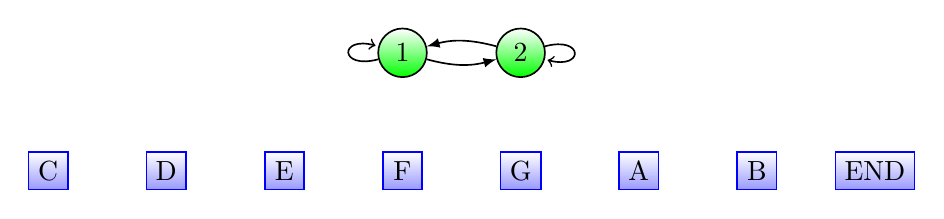
\begin{tikzpicture}[-latex, auto, node distance = 1.5cm and 1.5cm, on grid,
                    semithick,
                    state/.style = {circle,
                                    top color = white,
                                    bottom color = black!80,
                                    draw,
                                    black,
                                    text = black,
                                    minimum width = 0.5 cm},
                    obs/.style   = {rectangle,
                                    top color = white,
                                    bottom color = blue!40,
                                    draw,
                                    blue,
                                    text = black,
                                    minimum width = 0.5 cm}]

\node[state] (s1) [bottom color = green] {1};
\node[state] (s2) [bottom color = green, right = of s1] {2};

\node[obs] (F) [below = of s1] {F};
\node[obs] (G) [below = of s2] {G};


\node[obs] (E) [left = of F] {E};
\node[obs] (D) [left = of E] {D};
\node[obs] (C) [left = of D] {C};
\node[obs] (A) [right = of G] {A};
\node[obs] (B) [right = of A] {B};
\node[obs] (END) [right = of B] {END};

\path (s1) edge [loop left] (s1);
\path (s2) edge [loop right]  (s2);

\path (s1) edge [bend right = 15] (s2);
\path (s2) edge [bend right = 15] (s1);

\end{tikzpicture}
}


\newcommand{\transitiontypes}{
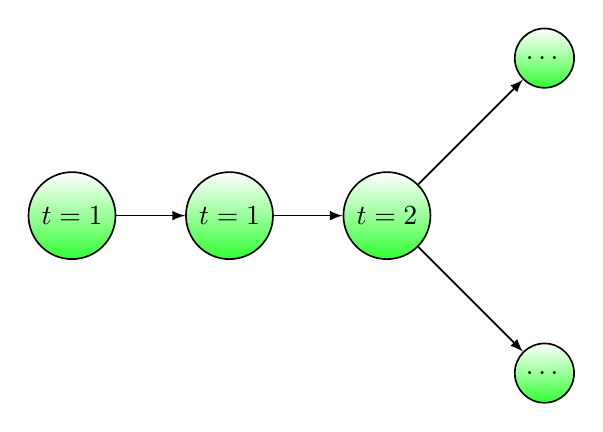
\begin{tikzpicture}[-latex, auto, node distance = 2cm and 2cm, on grid,
                    semithick,
                    state/.style = {circle,
                                    top color = white,
                                    bottom color = green!80,
                                    draw,
                                    black,
                                    text = black,
                                    minimum width = 0.5 cm},
                    obs/.style   = {rectangle,
                                    top color = white,
                                    bottom color = blue!40,
                                    draw,
                                    blue,
                                    text = black,
                                    minimum width = 0.5 cm}]

\node[state] (s1) {$t = 1$};
\node[state] (s2) [right = of s1] {$t = 1$};
\node[state] (s3) [right = of s2] {$t = 2$};
\node[state] (s4) [above right = of s3] {\ldots};
\node[state] (s5) [below right = of s3] {\ldots};

\path (s1) edge (s2);
\path (s2) edge (s3);
\path (s3) edge (s4);
\path (s3) edge (s5);

\end{tikzpicture}
}

\newcommand{\emissiontypes}{
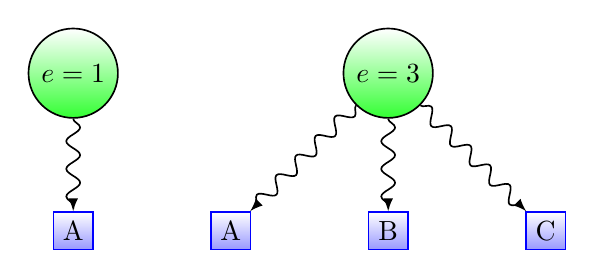
\begin{tikzpicture}[-latex, auto, node distance = 2cm and 2cm, on grid,
                    semithick,
                    state/.style = {circle,
                                    top color = white,
                                    bottom color = green!80,
                                    draw,
                                    black,
                                    text = black,
                                    minimum width = 0.5 cm},
                    obs/.style   = {rectangle,
                                    top color = white,
                                    bottom color = blue!40,
                                    draw,
                                    blue,
                                    text = black,
                                    minimum width = 0.5 cm}]

\node[state] (A) {$e = 1$};
\node[state] (B) [right = of A, xshift = 2cm] {$e = 3$};


\node[obs] (A1) [below = of A] {A};

\node[obs] (B2) [below = of B] {B};
\node[obs] (B1) [left = of B2] {A};
\node[obs] (B3) [right = of B2] {C};

\path[decoration={snake, post length=2pt}] (A) edge[decorate] (A1);

\path[decoration={snake, post length=2pt}] (B) edge[decorate] (B1);
\path[decoration={snake, post length=2pt}] (B) edge[decorate] (B2);
\path[decoration={snake, post length=2pt}] (B) edge[decorate] (B3);

\end{tikzpicture}
}